\chapter{声音、量子振子与第二定律}

\lectureoverview{第二定律是最终目标，但有两个具体计算为其铺路。声速检验热力学导数如何变成可观测的运动。谐振子随后揭示经典能量均分在刚性自由度上的失效，并展示量子力学如何逐个激活模式。我们最后回到可逆微观动力学与熵增之间的表面冲突，利用相空间流、粗粒化、混沌和回归，把第二定律表述为一条压倒性地可能的定律，而不是一条毫无例外的力学禁令。}

\section{关于第二定律的一个承诺}

核心问题容易陈述，却难以解释。牛顿方程是可逆的：如果某个微观历史被允许，那么时间反演的历史也被允许。然而第二定律说宏观过程有一个优选方向，其特征是熵通常增加。我们会谈到这一张力，但不是立刻。最好先看到统计力学产生具体信息，然后在一个初等计算中遇到那个迫使经典物理让位于量子物理的历史谜题。

第一个例子是数值性的，而且刻意粗糙：估计稀薄气体中的声速。第二个在其假设范围内是精确的：计算热浴中谐振子的平均能量。振子将引导我们从能量均分走向量子化能级，从一个模式走向无穷多个模式，最后回到多粒子系统忘记其初始状态意味着什么这一问题。

\section{声速的分子尺度}

想象稀薄气体中有一个小的过密区域。它之所以扩散，是因为分子离开拥挤区域，所以其传播速度应与分子速度相当。能量均分给出一个分子的动能，
\begin{equation}
 \frac{3}{2}k_B T
 =\frac{1}{2}m\expect{v^2},
 \qquad
 \expect{v^2}=\frac{3k_B T}{m}.
 \label{eq:sm7-molecular-speed}
\end{equation}
这里温度从绝对零度起量，并且由于我们想要实验室单位，\(k_B\) 已被恢复。这个论证只是一个尺度估计：分子的均方根速度本身并不是集体声波的速度。

更系统的推导考虑一小块气体。相对两面上的压力不等会施加一个净力，而其加速度与质量密度成反比。结果具有如下形式
\begin{equation}
 c_s^2=
 \left(\frac{\partial P}{\partial \rho_m}\right)_{\cal C},
 \qquad
 \rho_m=m\rho,
 \label{eq:sm7-sound-general}
\end{equation}
其中 \(\rho\) 是数密度，下标 \({\cal C}\) 指明扰动所遵循的热力学条件。板书计算使用
\begin{equation}
 P=\rho k_B T
 \quad\Longrightarrow\quad
 \frac{1}{m}
 \left(\frac{\partial P}{\partial\rho}\right)_T
 =\frac{k_B T}{m}.
 \label{eq:sm7-sound-isothermal}
\end{equation}
这是等温声速估计。它与 \eqref{eq:sm7-molecular-speed} 相差一个因子 \(3\)（在速度平方中），或者说在速度中相差 \(\sqrt{3}\)。

\begin{figure}[t]
\centering
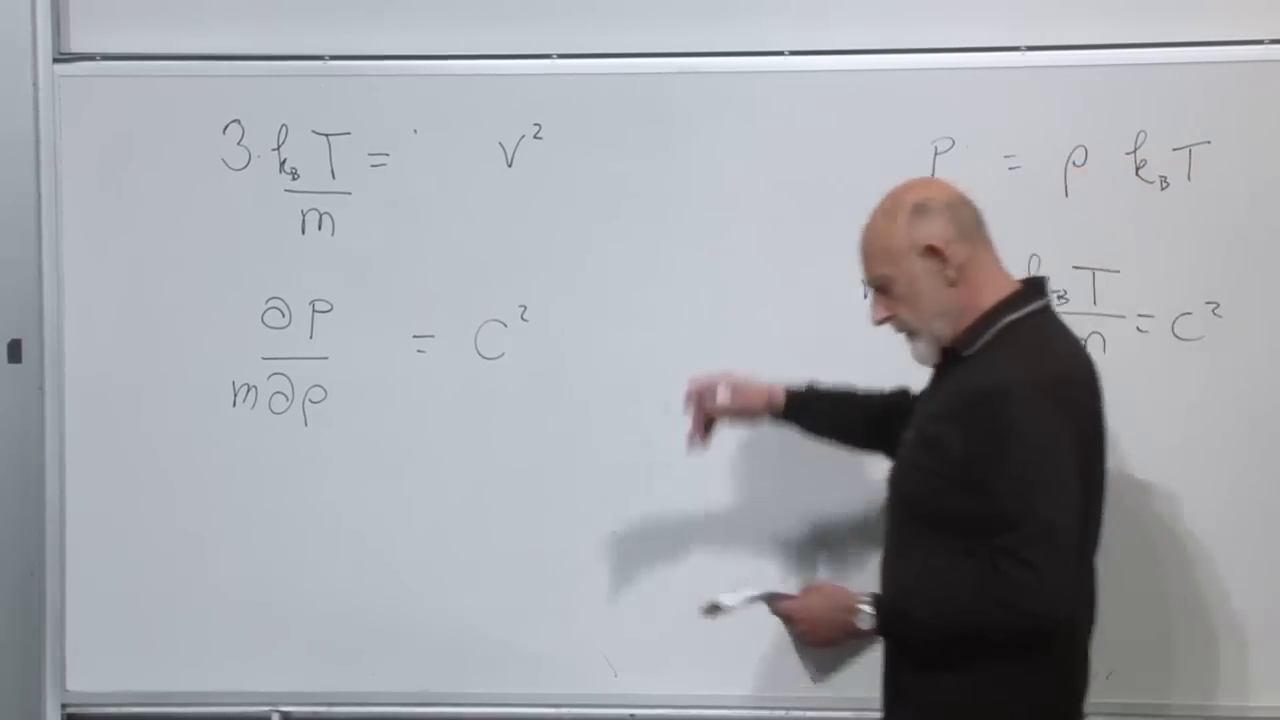
\includegraphics[width=0.90\textwidth]{lecture_07_figure_02.png}
\caption{分子速度估计、压力导数以及理想气体代换一起展示。}
\lectureframe{00:08:55}
\end{figure}

有一个重要的修正。小振幅声波压缩和稀疏气体的速度通常快于热量在相邻气体元之间流动的速度。因此局部运动近似为绝热的，而不是等温的：
\begin{equation}
 c_s^2=
 \left(\frac{\partial P}{\partial\rho_m}\right)_S.
 \label{eq:sm7-sound-adiabatic}
\end{equation}
对于绝热指数为 \(\gamma\) 的理想气体，
\begin{equation}
 P\rho_m^{-\gamma}=\text{constant},
 \qquad
 c_s^2=\gamma\frac{P}{\rho_m}
       =\gamma\frac{k_B T}{m}.
 \label{eq:sm7-sound-ideal-adiabatic}
\end{equation}
对于室温下的双原子空气，\(\gamma\simeq 7/5\)。因此，固定温度的计算是有用的初步估计，而绝热导数提供了物理上恰当的修正。

使用粗略值
\begin{equation}
\begin{aligned}
 k_B&\simeq1.3\times10^{-23}\ {\rm J\,K^{-1}},
 &T&\simeq300\ {\rm K},\\
 m_{\rm air}&\simeq4\times10^{-26}\ {\rm kg}.&&
\end{aligned}
 \label{eq:sm7-air-data}
\end{equation}
分子估计约为 \(500\ {\rm m\,s^{-1}}\)。这里的温度必须是开尔文绝对温度，而不是像华氏度那样的偏移标度。熟悉的声速约为 \(300\ {\rm m\,s^{-1}}\)，而绝热理想气体公式在室温下给出约 \(340\ {\rm m\,s^{-1}}\)。因此，粗略计算找到了正确的物理尺度。

\begin{figure}[t]
\centering
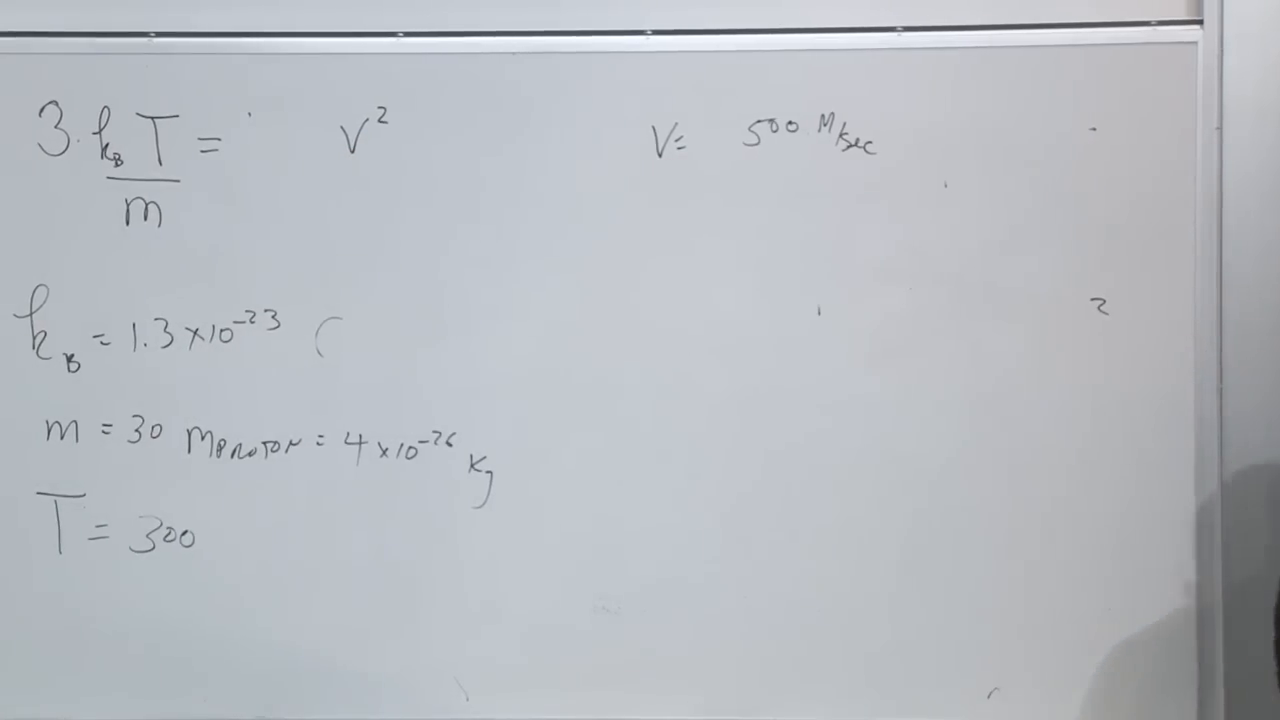
\includegraphics[width=0.90\textwidth]{lecture_07_figure_03.png}
\caption{使用玻尔兹曼常数、接近 \(30\) 个质子质量的有效分子质量以及 \(T\simeq300\ {\rm K}\) 对室温空气所作的估计。}
\lectureframe{00:10:55}
\end{figure}

早在有微观解释可用之前，人们就可以通过测量压力随密度的变化来确定声速。统计论证补充了一个引人注目的解释：由此得到的宏观速度由单个分子的热速度决定。

\begin{classroomqa}
\audiencequestion{分子质量中是否应当计入中子，而氮的数值\(14\)是否只计质子？}
\lecturerresponse{所引用的原子量已经计入了质子和中子。分子氮含有两个原子，其原子量约为\(14\)，因此其质量约为\(28\)个质子质量；对于这一估算，将\(28\)取整为\(30\)已经足够。
\lecturetimestamp{00:10:58--00:11:16}}
\end{classroomqa}

\begin{classroomqa}
\audiencequestion{因子\(3\)来自三个平动方向，而声波沿一个方向传播。这是否应当去掉因子\(3\)？}
\lecturerresponse{它正确地提醒我们，不应把三维的分子均方根速率与一维的传播速率等同起来。开头的论证只是一个数量级图像。一个受控的答案来自压强导数，并结合适用于该波的热力学条件。
\lecturetimestamp{00:11:12--00:12:00}}
\end{classroomqa}

\begin{classroomqa}
\audiencequestion{该导数是否假定了波传播过程中温度保持不变？}
\lecturerresponse{所展示的理想气体代换确实如此。对于极小的扰动，固定温度是一个合理的临时估计；标准的改进是，普通声波近似为绝热的，这会把等温导数替换为\(\left(\partial P/\partial\rho_m\right)_S\)。
\lecturetimestamp{00:12:59--00:14:01}}
\end{classroomqa}

\begin{classroomqa}
\audiencequestion{如果压强和密度的变化都很小，是否就使它们的导数很小？}
\lecturerresponse{不。导数是在无穷小极限下两个小变化量之比。\(\delta P\)和\(\delta\rho\)都可以很小，而\(\delta P/\delta\rho\)仍保持有限，并决定波速。
\lecturetimestamp{00:14:03--00:14:23}}
\end{classroomqa}

\begin{classroomqa}
\audiencequestion{当气体被压缩时，声速是否应当升高，就像从气体过渡到液体或固体时那样？}
\lecturerresponse{是的。导数是在所考虑的状态下求值的，而\(P(\rho,T)\)不必保持线性。当分子被挤压得彼此靠近时，状态方程变为非理想的，\(\partial P/\partial\rho\)可以显著增大。
\lecturetimestamp{00:14:25--00:15:13}}
\end{classroomqa}

\begin{classroomqa}
\audiencequestion{数值\(500\ {\rm m\,s^{-1}}\)能否在任意压强下使用？}
\lecturerresponse{不能。它属于低密度范围，在该范围内理想气体方程是有用的近似。一旦密度的更高次幂进入\(P(\rho,T)\)，导数、从而声速就依赖于压强和密度。
\lecturetimestamp{00:15:14--00:16:29}}
\end{classroomqa}

\begin{classroomqa}
\audiencequestion{随着密度增大，声波以大致分子速率传播的原始图像是否也会失效？}
\lecturerresponse{很可能。该图像是为稀薄气体量身定制的。在高密度下，集体相互作用变得越来越重要，这正是状态方程导数成为更一般描述的原因。
\lecturetimestamp{00:16:32--00:16:53}}
\end{classroomqa}

\begin{classroomqa}
\audiencequestion{为什么氮分子质量写成大约\(30\)个质子质量，而不是\(28\)？}
\lecturerresponse{只需要与估算相称的数值精度，因此将\(28\)取整为\(30\)。将原来的\(500\ {\rm m\,s^{-1}}\)估计值除以\(\sqrt{3}\simeq1.7\)也使其接近\(300\ {\rm m\,s^{-1}}\)，尽管绝热导数是计算修正的受控方法。
\lecturetimestamp{00:16:54--00:17:27}}
\end{classroomqa}

\section{热浴中的一个经典振子}

现在我们用一个谐振子代替自由平动的分子，并把其他一切视为热浴。弹簧上的质量块是最直接的图像，但该模型要广泛得多。电磁腔模会振荡；晶体中的原子会振荡；几乎任何稍微偏离平衡的稳定系统，在最低阶上都作简谐运动。

以\(x\)为偏离平衡的位移，动量为\(p\)，质量为\(m\)，弹簧常数为\(\kappa\)，哈密顿量为
\begin{equation}
 H(x,p)=\frac{p^2}{2m}+\frac{\kappa x^2}{2},
 \qquad
 \omega=\sqrt{\frac{\kappa}{m}}.
 \label{eq:sm7-classical-hamiltonian}
\end{equation}
热浴固定\(T\)，从这一点起我们再次使用\(k_B=1\)，因此\(\beta=1/T\)。与室温平衡的振子温度接近\(300\ {\rm K}\)；浸入液氦中的振子温度只有几开尔文。一个假想的弹簧若放在太阳中心，就不会作为弹簧存活下来，但这个例子清楚地说明了环境的作用。玻尔兹曼权重因子分解为：
\begin{equation}
 e^{-\beta H}
 =e^{-\beta p^2/(2m)}
  e^{-\beta\kappa x^2/2}.
 \label{eq:sm7-factorized-weight}
\end{equation}

\begin{figure}[t]
\centering
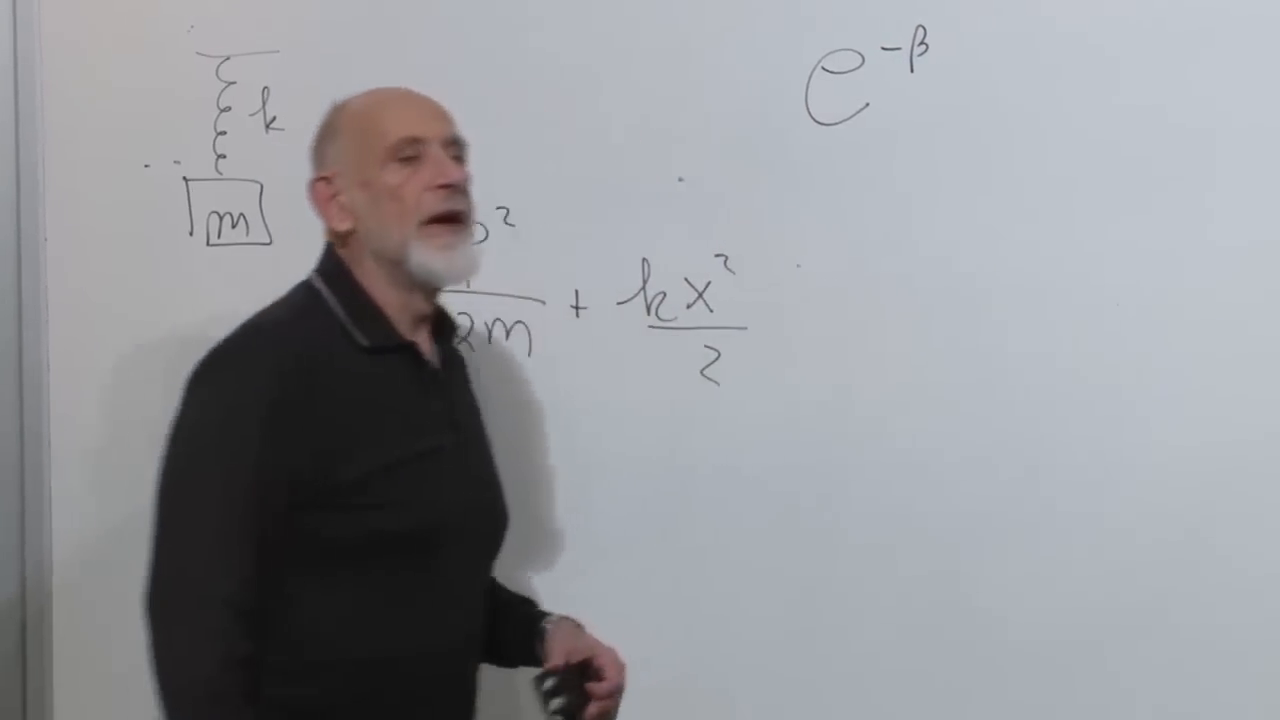
\includegraphics[width=0.90\textwidth]{lecture_07_figure_04.png}
\caption{弹簧-质量振子及其动能加势能的哈密顿量。}
\lectureframe{00:20:55}
\end{figure}

与自由气体不同，位置积分并不仅仅给出容器体积。恢复势对每个位移进行加权：
\begin{equation}
 Z_{\rm cl}
 =\frac{1}{h}\int_{-\infty}^{\infty}dp
             \int_{-\infty}^{\infty}dx\,
 e^{-\beta p^2/(2m)}
 e^{-\beta\kappa x^2/2}.
 \label{eq:sm7-classical-z}
\end{equation}
因子\(1/h\)使一维经典配分函数无量纲。它在板书计算中被略去，因为它与\(\beta\)无关，不可能影响平均能量。

\begin{figure}[t]
\centering
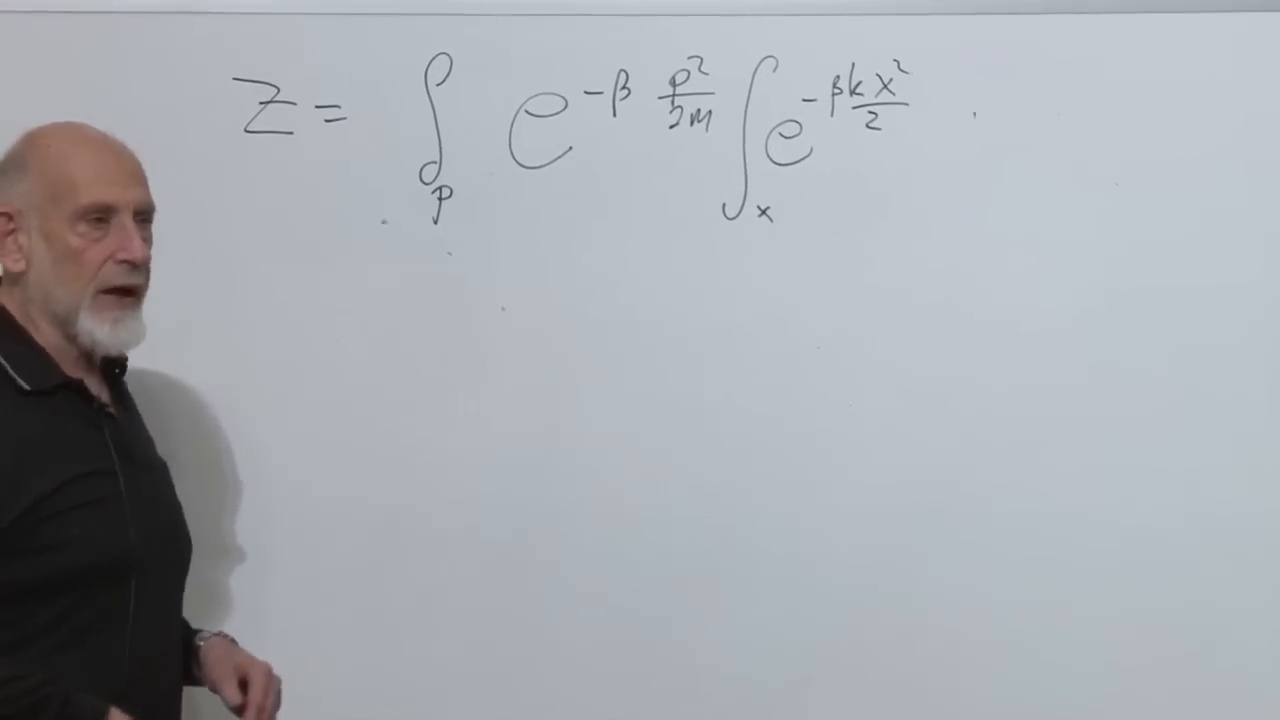
\includegraphics[width=0.90\textwidth]{lecture_07_figure_05.png}
\caption{经典振子配分函数分解为其动量与位移的高斯积分。}
\lectureframe{00:22:55}
\end{figure}

对于动量积分，令
\begin{equation}
 q=\sqrt{\frac{\beta}{2m}}\,p,
 \qquad
 dp=\sqrt{\frac{2m}{\beta}}\,dq.
 \label{eq:sm7-p-gaussian-substitution}
\end{equation}
对于位置积分，令
\begin{equation}
 y=\sqrt{\frac{\beta\kappa}{2}}\,x,
 \qquad
 dx=\sqrt{\frac{2}{\beta\kappa}}\,dy.
 \label{eq:sm7-x-gaussian-substitution}
\end{equation}
由于\(\int_{-\infty}^{\infty}e^{-u^2}\,du=\sqrt{\pi}\)，板书上所用的未归一化相空间积分为
\begin{equation}
 \int dp\,dx\,e^{-\beta H}
 =\frac{2\pi}{\beta}\sqrt{\frac{m}{\kappa}}
 =\frac{2\pi}{\beta\omega}.
 \label{eq:sm7-classical-z-unnormalized}
\end{equation}
恢复相空间元胞后，
\begin{equation}
 Z_{\rm cl}=\frac{2\pi}{h\beta\omega}
           =\frac{1}{\beta\hbar\omega}.
 \label{eq:sm7-classical-z-normalized}
\end{equation}

只有\(\beta\)依赖关系对能量有影响：
\begin{equation}
 \begin{aligned}
 \log Z_{\rm cl}&=\text{constant}-\log\beta,\\
 \expect{H}
 &=-\frac{\partial\log Z_{\rm cl}}{\partial\beta}\\
 &=\frac{1}{\beta}=T.
 \end{aligned}
 \label{eq:sm7-classical-energy}
\end{equation}

\begin{figure}[t]
\centering
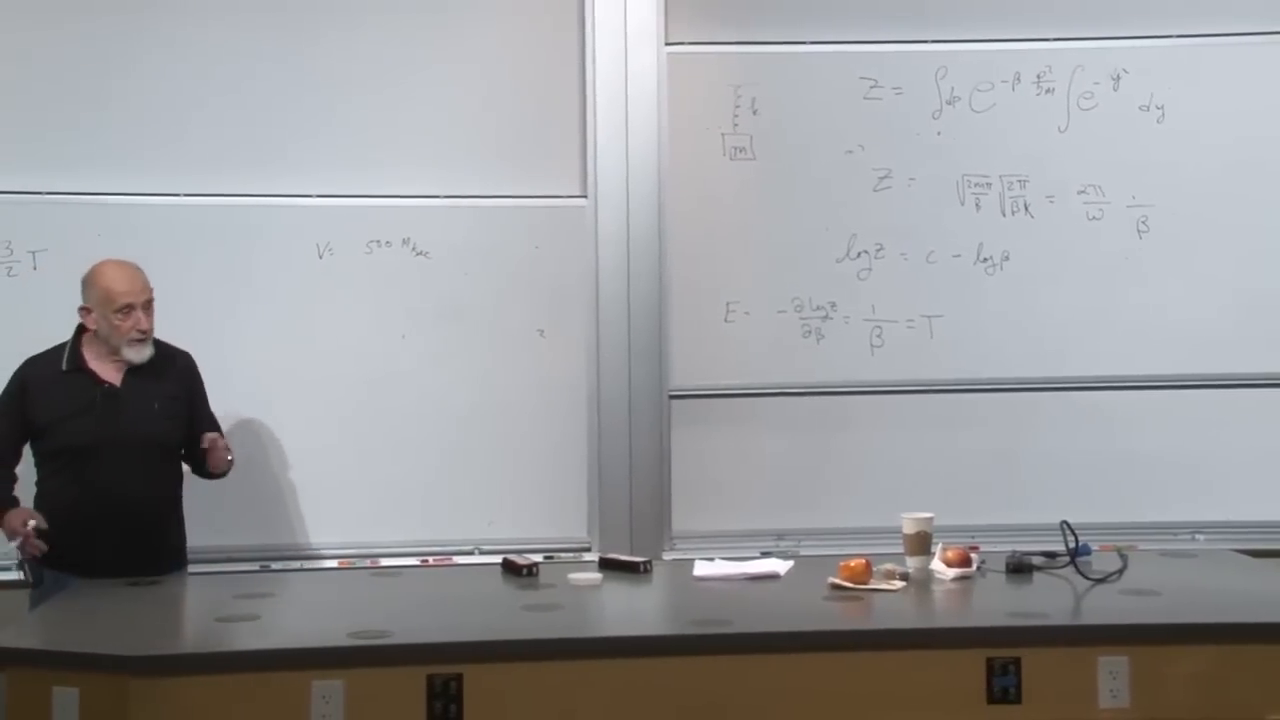
\includegraphics[width=0.90\textwidth]{lecture_07_figure_06.png}
\caption{右侧黑板上的完整经典推导链：高斯因子化、\(Z\propto(\beta\omega)^{-1}\)以及\(\expect{H}=1/\beta=T\)。}
\lectureframe{00:30:15}
\end{figure}

没有因子\(3\)，因为这是一个空间振子。也不存在剩余的因子\(1/2\)，因为有两个独立的二次项。每个高斯积分贡献\(T/2\)：
\begin{equation}
 \expect{K}=\frac{T}{2},
 \qquad
 \expect{U}=\frac{T}{2},
 \qquad
 \expect{H}=T.
 \label{eq:sm7-equipartition-oscillator}
\end{equation}
这是能量均分最实用的形式：经典哈密顿量中每一个独立的二次项都贡献\(T/2\)。

答案与\(m\)和\(\kappa\)都无关。运动本身确实依赖于这些参数：
\begin{equation}
 \expect{p^2}=mT,
 \qquad
 \expect{x^2}=\frac{T}{\kappa},
 \qquad
 \expect{\dot{x}^2}=\frac{T}{m}.
 \label{eq:sm7-classical-fluctuations}
\end{equation}
因此较重的质量运动得更慢，较硬的弹簧振幅更小，尽管平均能量仍为\(T\)。当\(\kappa\)被取得极大时，这就变得令人不安。硬得无法运动的弹簧应当看起来像冻结的约束，然而经典能量均分仍然赋予它能量\(T\)。

\begin{classroomqa}
\audiencequestion{当\(\kappa\to\infty\)时，配分函数趋于零。它的对数怎么还能使用？}
\lecturerresponse{保持\(\kappa\)有限但任意大。它对\(\log Z\)的贡献是可加的且与\(\beta\)无关，因此对\(\beta\)求导仍然给出\(T\)。这种极限下的不适感是真实的：经典计算内部自洽，但它遗漏了自然界对于极硬振子所必需的一个特征。
\lecturetimestamp{00:34:01--00:34:54}}
\end{classroomqa}

\begin{classroomqa}
\audiencequestion{理想气体配分函数需要一个\(N!\)。这里是否应有类似的阶乘？}
\lecturerresponse{没有。我们研究的是一个指定的振子，而不是对\(N\)个全同粒子进行排列。对于许多独立的标记模式，配分函数相乘。不可区分性因子属于另一个计数问题。
\lecturetimestamp{00:35:03--00:35:40}}
\end{classroomqa}

\section{为什么经典能量均分是一场危机}

真实分子并非无结构的点。双原子分子包含一个可以振动的键，因而有一个内部振子。朴素的经典计数即使在常温下也会给该模式分配额外的热能。在一个刻意简化的示意性计数中，激活一个振动振子会把\(3T/2\)的能量推向\(5T/2\)。精确的热容记账还必须包括转动自由度，并区分能量与其对温度的导数。决定性的实验事实更简单：刚性内部模式在低温下并未像经典能量均分所要求的那样作出贡献。

人们可以否认分子具有内部结构，但这是荒谬的；或者承认经典力学缺少一个要素。这个要素就是量子力学。我们只需要它极少的一部分：谐振子具有等间距的能级。

\section{量子振子}

首先移动能量原点，将激发谱写为
\begin{equation}
 E_n^{\rm exc}=n\hbar\omega,
 \qquad n=0,1,2,\ldots.
 \label{eq:sm7-shifted-spectrum}
\end{equation}
配分函数现在是一个真正的求和，而不是相空间积分：
\begin{align}
 Z_{\rm exc}
 &=\sum_{n=0}^{\infty}e^{-\beta n\hbar\omega} \notag\\
 &=1+x+x^2+\cdots
  =\frac{1}{1-x},
 \qquad x=e^{-\beta\hbar\omega}, \notag\\
 &=\frac{1}{1-e^{-\beta\hbar\omega}}.
 \label{eq:sm7-quantum-z}
\end{align}

\begin{figure}[t]
\centering
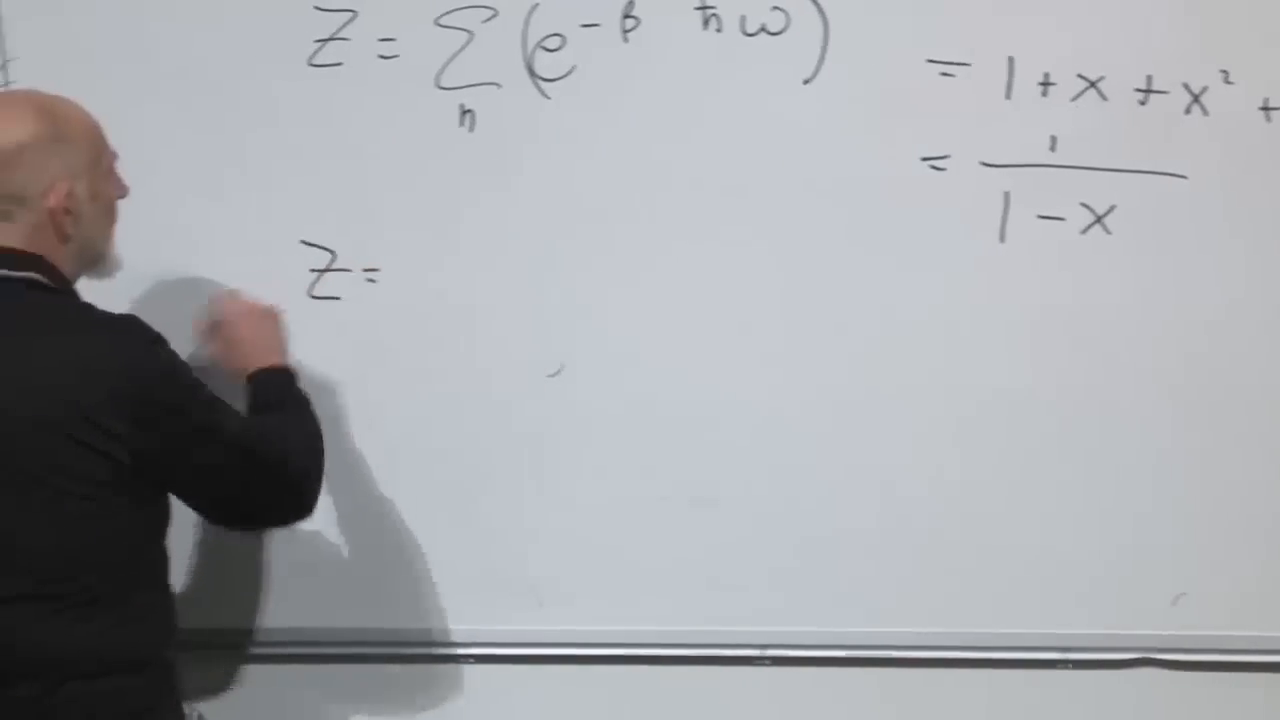
\includegraphics[width=0.90\textwidth]{lecture_07_figure_07.png}
\caption{等间距能级以及量子振子配分函数的几何级数求值。}
\lectureframe{00:42:05}
\end{figure}

求导给出平均激发能量：
\begin{align}
 E_{\rm exc}
 &=-\frac{\partial\log Z_{\rm exc}}{\partial\beta}
  =-\frac{1}{Z_{\rm exc}}
    \frac{\partial Z_{\rm exc}}{\partial\beta}
 \notag\\
 &=\hbar\omega\,
   \frac{e^{-\beta\hbar\omega}}
        {1-e^{-\beta\hbar\omega}}
  =\frac{\hbar\omega}{e^{\beta\hbar\omega}-1}.
 \label{eq:sm7-quantum-energy}
\end{align}

\begin{figure}[t]
\centering
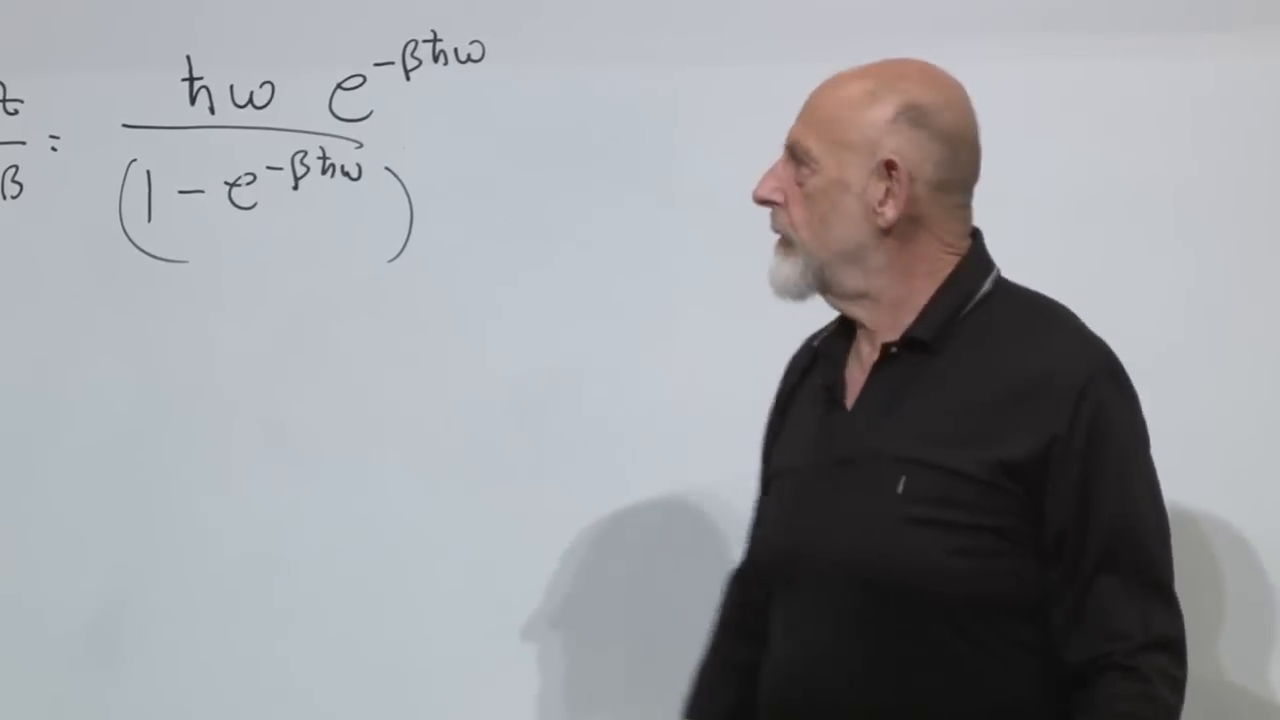
\includegraphics[width=0.90\textwidth]{lecture_07_figure_08.png}
\caption{由量子配分函数的\(\beta\)导数得到的热激发能量。}
\lectureframe{00:46:05}
\end{figure}

\subsection{高温}

当\(\beta\hbar\omega\ll1\)时，
\begin{equation}
 e^{-\beta\hbar\omega}
 =1-\beta\hbar\omega
  +O\!\left((\beta\hbar\omega)^2\right).
 \label{eq:sm7-high-t-expansion}
\end{equation}
\eqref{eq:sm7-quantum-energy}的分子趋于\(\hbar\omega\)，而分母在领头阶为\(\beta\hbar\omega\)。因此
\begin{equation}
 E_{\rm exc}\simeq\frac{1}{\beta}=T.
 \label{eq:sm7-high-t-energy}
\end{equation}
当许多能级间距都落在热能之内时，量子答案恢复经典能量均分。

\subsection{低温}

当 \(\beta\hbar\omega\gg1\) 时，指数项极小：
\begin{equation}
 E_{\rm exc}
 \simeq\hbar\omega e^{-\beta\hbar\omega}.
 \label{eq:sm7-low-t-energy}
\end{equation}
振子的热激发受到指数抑制。在平移后的约定中它几乎为零；物理上的零点能将在下文恢复。

\begin{figure}[t]
\centering
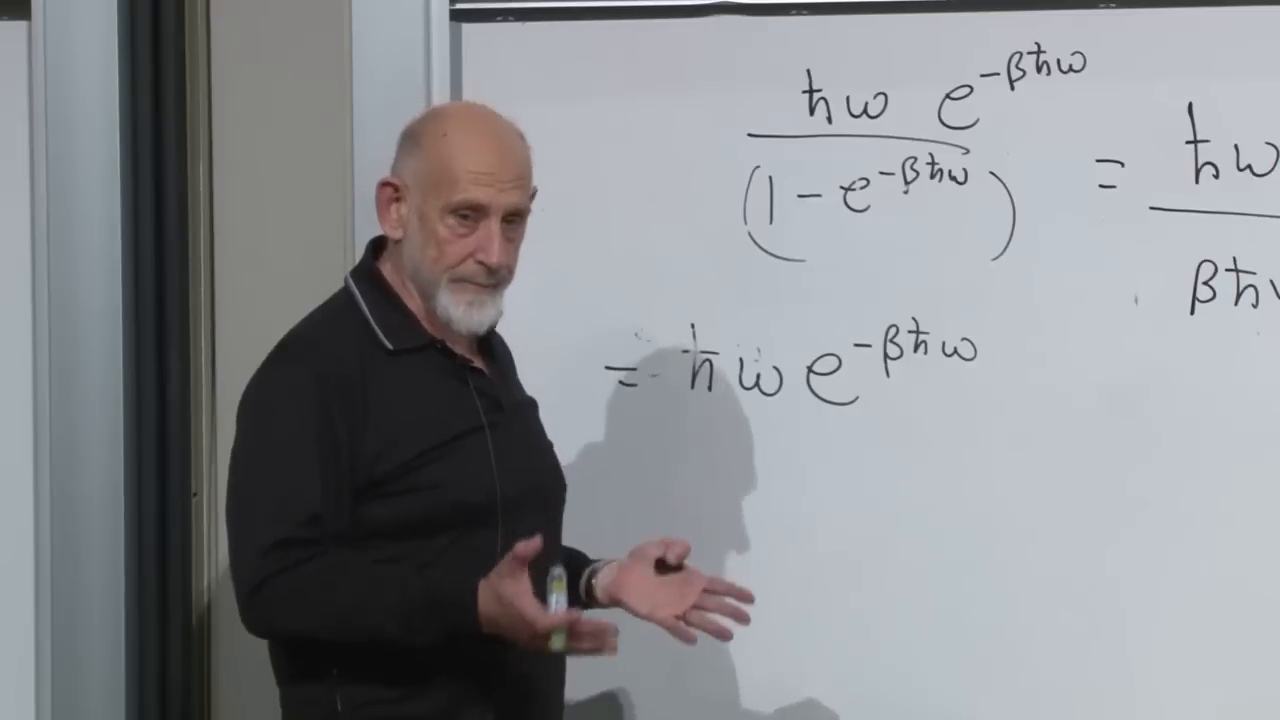
\includegraphics[width=0.90\textwidth]{lecture_07_figure_09.png}
\caption{低温展开：第一热激发受到 \(e^{-\beta\hbar\omega}\) 的抑制。}
\lectureframe{00:51:55}
\end{figure}

交叉发生在
\begin{equation}
 \beta\hbar\omega\sim1,
 \qquad\text{or equivalently}\qquad
 T\sim\hbar\omega.
 \label{eq:sm7-crossover}
\end{equation}
这一条件有直接的含义。经典能量均分给出振子能量 \(T\)。当该尺度低于一个能级间距时，量子效应便不可避免。因此
\begin{equation}
\begin{aligned}
 \hbar\omega\gg T&:\quad \text{frozen and quantum},\\
 \hbar\omega\ll T&:\quad \text{active and classical}.
\end{aligned}
 \label{eq:sm7-regimes}
\end{equation}
更硬的弹簧有更大的 \(\omega=\sqrt{\kappa/m}\)，因此需要更高的温度才能表现为经典行为。

\section{加热物质时自由度显现}

在低温下，双原子分子在热学上可以像一个点粒子，因为其刚性键振动被冻结。当 \(T\) 升高越过 \(\hbar\omega\) 时，振动模式被激活。转动模式可能在更低的尺度上激活；更高的温度会揭示更多内部运动，并最终使原子电离。加热并非仅仅向一份固定的模式清单中注入更多能量。它揭示出在较低温度下不可见的自由度。

一个假想的嵌套分子能更清楚地说明这一点。两个原子由一根刚性弹簧连接，而其中一个看似原子的部分本身又是一对由更硬弹簧连接的原子。在低 \(T\) 下，两种结构都看起来像点。在第一个阈值处，外层振动出现；在第二个阈值处，内部结构出现。系统的复杂性随着能量尺度被逐级揭示。

\begin{classroomqa}
\audiencequestion{一旦振子已处于经典区域，继续加热会使弹簧变紧还是改变其频率？}
\lecturerresponse{不会。弹簧常数和频率保持不变。更高的温度产生更大的典型动量和振幅，因而能量更大。刚度决定经典定律从哪个温度开始，而不是弹簧随温度变紧。
\lecturetimestamp{01:03:17--01:05:11}}
\end{classroomqa}

\subsection{晶体与爱因斯坦的比热}

晶体包含大量振动模式。经典能量均分给每个活跃振子分配 \(T\) 量级的能量，因此高估了低温热容。爱因斯坦的 1907 模型以量子力学方式处理晶体振动，并说明了为什么在热能未达到其能级间距之前这些振动会受到抑制。更精确的固态模型允许模式频率有一个分布，但冻结原理在爱因斯坦的计算中已经存在。

\begin{classroomqa}
\audiencequestion{这是爱因斯坦获得诺贝尔奖的工作吗？它是否只在量子力学建立之后才出现？}
\lecturerresponse{不是。诺贝尔奖的授奖说明涉及光电效应。比热模型发表于 1907，远在量子力学完整基础被理解之前。爱因斯坦接受并发展了关键的量子思想，尽管他后来反对成熟理论的某些方面。
\lecturetimestamp{00:58:38--01:03:16}}
\end{classroomqa}

\begin{classroomqa}
\audiencequestion{经典统计力学把对离散态的求和替换为对位置和动量的看似均匀的积分。是什么为这种态计数提供了依据？}
\lecturerresponse{最终的依据来自量子力学。在高温极限下，
\[
 Z_{\rm exc}\simeq\frac{1}{\beta\hbar\omega},
\]
这恰好与无量纲的经典结果 \eqref{eq:sm7-classical-z-normalized} 相符。当能级间距无法分辨时，相空间中的量子胞元就变成经典相空间测度。
\lecturetimestamp{00:59:38--01:03:06}}
\end{classroomqa}

\subsection{一根弦包含无穷多个振子}

小提琴弦或吉他弦分解为简正模式：基频、更高次谐波，以及越来越短的波长。数学上有无穷多个振子模式。如果经典能量均分给每一个模式分配能量 \(T\)，那么处于热平衡的弦将具有无穷大的能量。量子力学阻止了这种灾难。最短波长的模式具有最高频率，在任何有限温度下都保持冻结；随着 \(T\) 升高，越来越多的模式被激活。同样的逻辑后来将成为黑体辐射的基础。

\begin{figure}[t]
\centering
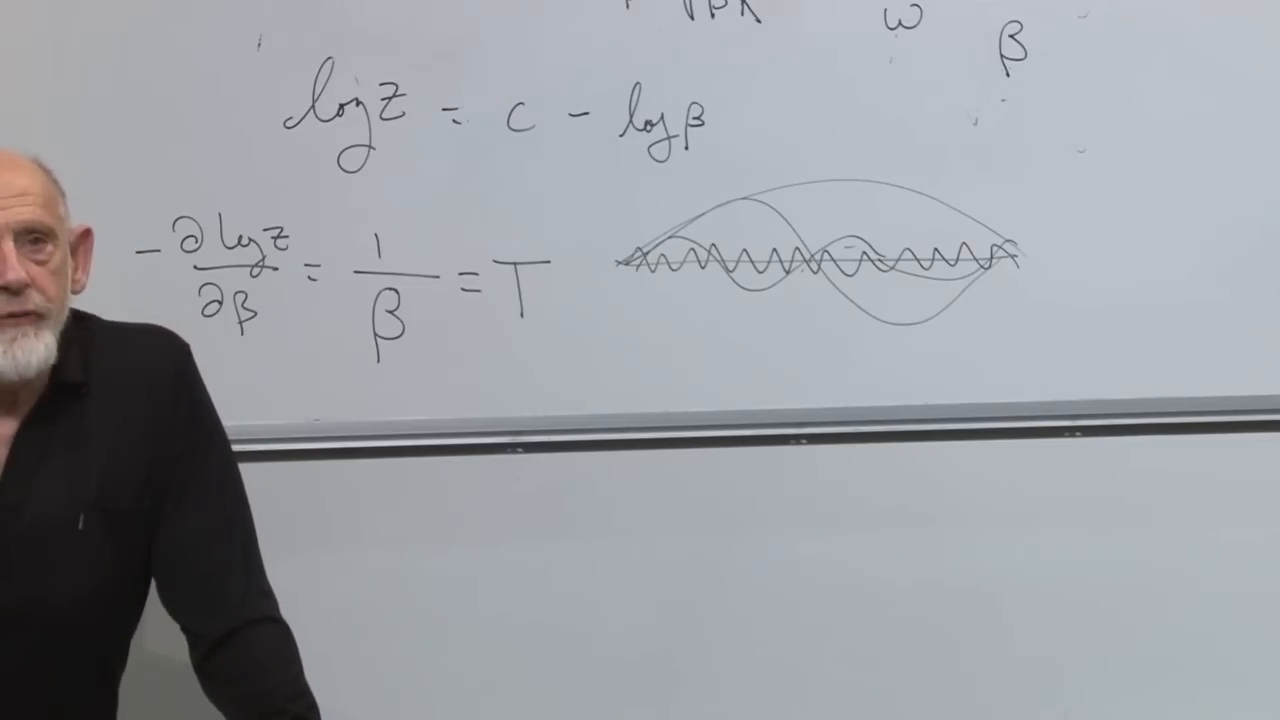
\includegraphics[width=0.90\textwidth]{lecture_07_figure_10.png}
\caption{叠加在弦上的若干简正模式，说明为什么连续弦是无穷多个谐振子的集合。}
\lectureframe{01:09:30}
\end{figure}

\begin{classroomqa}
\audiencequestion{量子到经典的过渡能否被直接观测到，加热又能否逆转低温行为？}
\lecturerresponse{能。晶体比热的温度依赖性使振动模式的冻结以及随后的激活变得可以明确测量。
\lecturetimestamp{01:09:11--01:10:13}}
\end{classroomqa}

\begin{classroomqa}
\audiencequestion{对于许多振子，我们是否对每个模式重复单振子配分函数？}
\lecturerresponse{对于独立模式，
\[
\begin{aligned}
 Z_{\rm tot}&=\prod_j Z_j,&
 \log Z_{\rm tot}&=\sum_j\log Z_j,\\
 E_{\rm tot}&=\sum_j E_j.&&
\end{aligned}
\]
满足\(\hbar\omega_j\gg T\)的模式对热贡献呈指数级小；低于该阈值的模式则有可观贡献。
\lecturetimestamp{01:10:14--01:11:00}}
\end{classroomqa}

\begin{classroomqa}
\audiencequestion{振子的零点能\(\hbar\omega/2\)怎么了？}
\lecturerresponse{物理能级为
\[
 E_n=\left(n+\frac12\right)\hbar\omega.
\]
因此
\[
 \begin{aligned}
 Z_{\rm phys}
 &=e^{-\beta\hbar\omega/2}Z_{\rm exc},\\
 E_{\rm phys}
 &=\frac{\hbar\omega}{2}
  +\frac{\hbar\omega}{e^{\beta\hbar\omega}-1}.
 \end{aligned}
\]
这一共同平移不改变能级概率、熵、热容或热激发能，但它确实使绝对平均能量平移了\(\hbar\omega/2\)。\(Z\)中的乘性因子依赖于\(\beta\)，因此当需要绝对能量时，不能将其丢弃。
\lecturetimestamp{01:11:08--01:11:37}}
\end{classroomqa}

\section{作为可逆性谜题的第二定律}

现在我们可以回到之前承诺要讨论的问题。第二定律说，普通的宏观演化是不可逆的，并且熵倾向于增加。微观的哈密顿演化是可逆的。一个对精确状态的可逆映射，如何能产生关于宏观状态的不可逆定律？

用高维相空间中的一个点来表示系统，
\[
 \Gamma=(q_1,\ldots,q_N,p_1,\ldots,p_N).
\]
我们的知识通常不是一个精确的点。假设它是紧致区域\(A\)上的均匀概率密度，其体积为\(\Omega_A\)：
\begin{equation}
 f(\Gamma)=
 \begin{cases}
  1/\Omega_A,&\Gamma\in A,\\
  0,&\Gamma\notin A.
 \end{cases}
 \label{eq:sm7-uniform-blob}
\end{equation}
在\(k_B=1\)的单位制下，其细粒化吉布斯熵为
\begin{equation}
 S_{\rm fine}
 =-\int d\Gamma\,f\log f
 =\log\Omega_A.
 \label{eq:sm7-blob-entropy}
\end{equation}
区域越小意味着信息越多、熵越低。这确定了符号：不确定性增加会扩大被占据的区域并提高\(\log\Omega_A\)。

\begin{figure}[t]
\centering
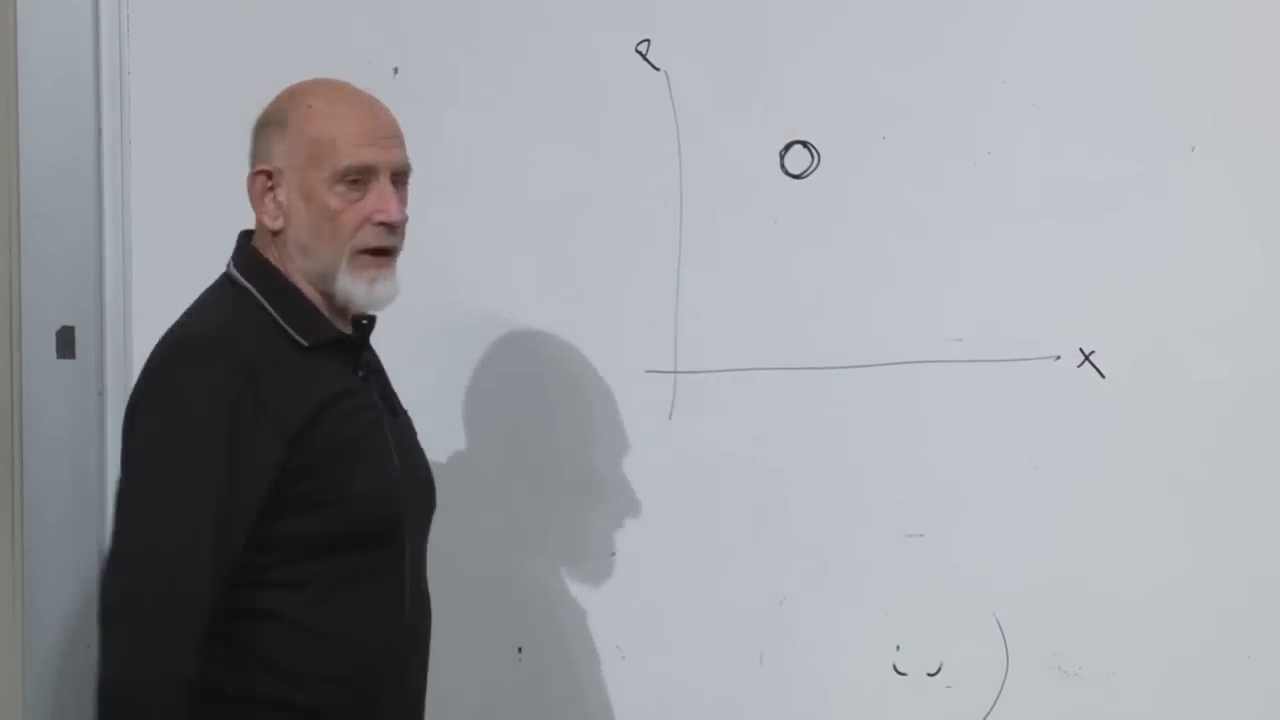
\includegraphics[width=0.90\textwidth]{lecture_07_figure_11.png}
\caption{完整位置-动量相空间的示意性二维切片中的一个紧致概率区域。}
\lectureframe{01:20:20}
\end{figure}

\begin{classroomqa}
\audiencequestion{系统是否受到物理约束而必须留在所画区域之内，它是否已经处于平衡？}
\lecturerresponse{不。该区域描述的是关于初始状态已知的信息，而不是相空间中的一堵墙。它不必是平衡分布。一个最初被限制在房间一角容器中的气体，就是特殊的非平衡信息的一个具体例子。
\lecturetimestamp{01:14:55--01:15:24}}
\end{classroomqa}

\section{刘维尔流与粗粒化增长}

刘维尔定理说，哈密顿流保持相空间体积。精确区域可以平移、拉伸、折叠并变得极其细薄，但
\begin{equation}
 \Omega_{A(t)}=\Omega_{A(0)},
 \qquad
 S_{\rm fine}(t)=S_{\rm fine}(0).
 \label{eq:sm7-liouville}
\end{equation}
其离散类比是状态的可逆置换。如果最初知道一个骰子处于两种状态之一，一对一的演化可以改变它们是哪两种状态，但不会改变可能性的数目。

真实的描述具有有限分辨率。量子力学提供了一个自然的相空间胞元，而经典实验即使不援引量子理论也具有有限的测量能力。在哈密顿流下，区域可以变成一条细长的蛇。如果相邻折叠之间的间隔低于分辨率尺度，我们就用粗粒胞元代替每个无法分辨的邻域。精确占据体积保持不变，但粗粒胞元的并集增大了：
\begin{equation}
 \Omega_{\rm coarse}(t)\geq\Omega_{A(t)},
 \qquad
 S_{\rm coarse}(t)=\log\Omega_{\rm coarse}(t).
 \label{eq:sm7-coarse-entropy}
\end{equation}

\begin{figure}[t]
\centering
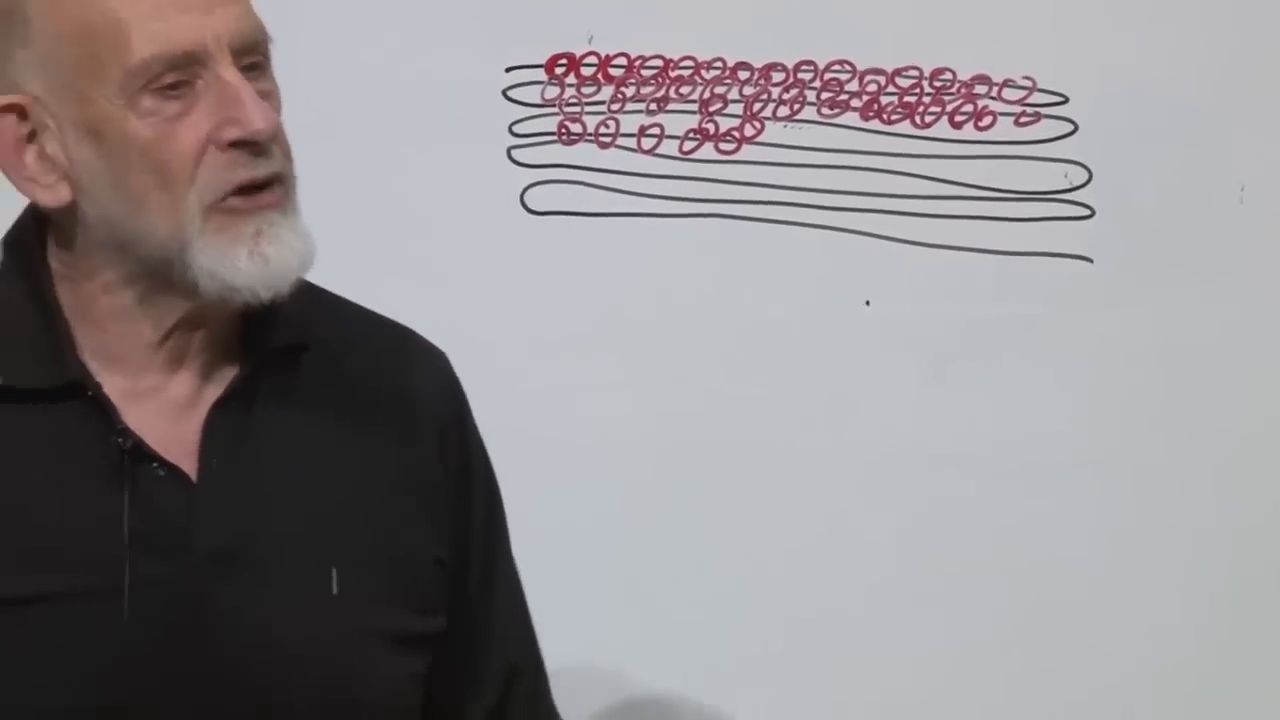
\includegraphics[width=0.90\textwidth]{lecture_07_figure_12.png}
\caption{通过有限分辨率胞元观察的保体积细丝。精确的黑色细丝保持其面积；红色粗粒胞元占据更大的有效区域。}
\lectureframe{01:22:10}
\end{figure}

\begin{classroomqa}
\audiencequestion{粗粒胞元发生重叠。这是否违反刘维尔定理？}
\lecturerresponse{不。刘维尔定理支配的是精确细丝，它保持一对一且保体积。重叠属于我们模糊的描述：我们已经丢弃了关于状态位于哪条细丝中的信息。
\lecturetimestamp{01:21:32--01:21:50}}
\end{classroomqa}

一个有用的类比是棉花。所有纤维的材料体积可以几乎保持不变，而一团被扯松的棉絮在无法分辨单根纤维的观察者看来却占据很大的表观体积。同样，相空间区域会长出越来越细的触须；那些触须又会长出更细的触须。任何固定的有限分辨率最终都无法跟上它们。

\begin{classroomqa}
\audiencequestion{熵是否只是在经典意义上看似增加，而量子力学通过施加基本的分辨率极限才使这种增加成为真实的？}
\lecturerresponse{粗粒化论证并不需要量子极限。熵同时指系统及其描述中所保留的宏观区分。在拥有无限微观信息时，细粒化熵是常数；在任何固定的有限分辨率下，混沌细丝最终变得无法分辨，粗粒化熵随之增加。
\lecturetimestamp{01:24:04--01:25:20}}
\end{classroomqa}

\section{混沌、有限的可达区域与平衡化}

对于盒中的气体，位置是有界的。在固定的有限总能量下，动量同样有界，即使全部能量暂时集中在一个粒子上也是如此。因此，在通常的约束假设下，动力学上可及的能量壳层具有有限测度。

\begin{figure}[t]
\centering
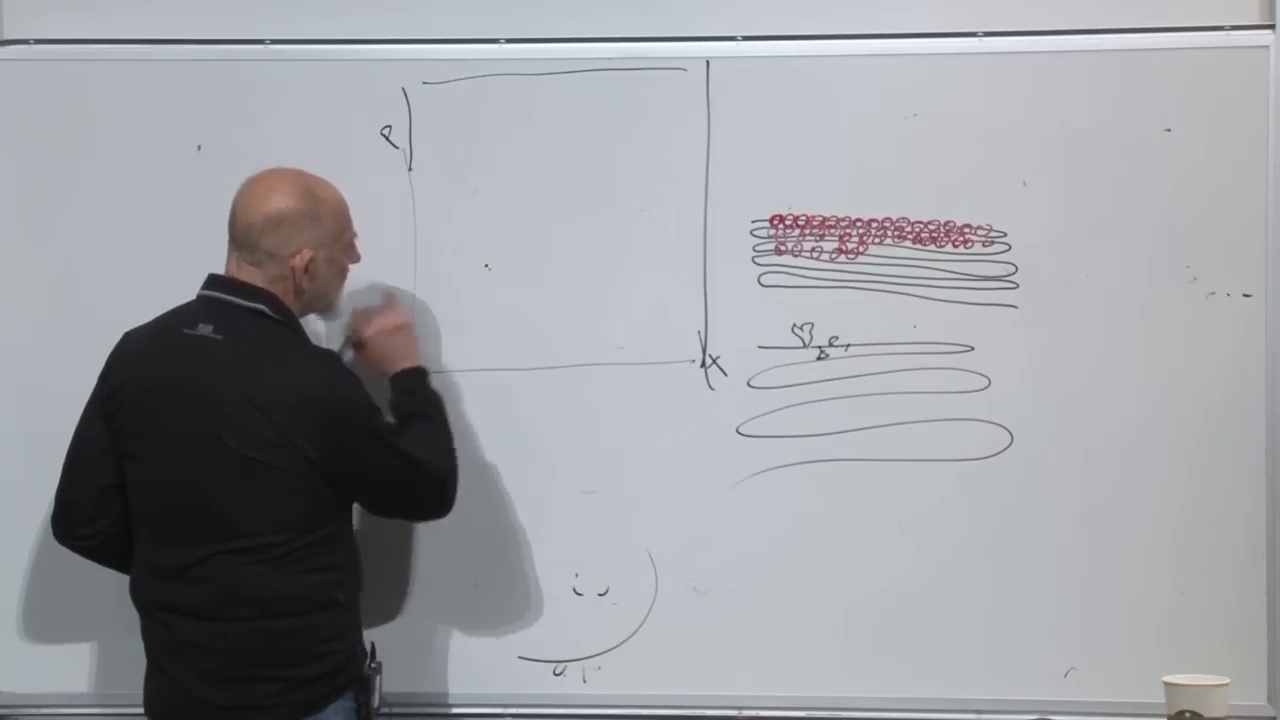
\includegraphics[width=0.90\textwidth]{lecture_07_figure_13.png}
\caption{有界的可及相空间区域，旁边是细丝及其粗粒化表示。}
\lectureframe{01:28:10}
\end{figure}

混沌系统中邻近的初始点在最初一段时间内遵循相似的历史，随后分离。在一次台球开球中，母球方向上一个不可察觉的变化会被复制到随后的碰撞中；差异不断累积，直到最终构型彼此无关。因此，整个初始斑块在可及区域中被拉伸和折叠。在有限分辨率下，它趋近于一种宽广、近乎均匀的平衡描述。

\begin{figure}[t]
\centering
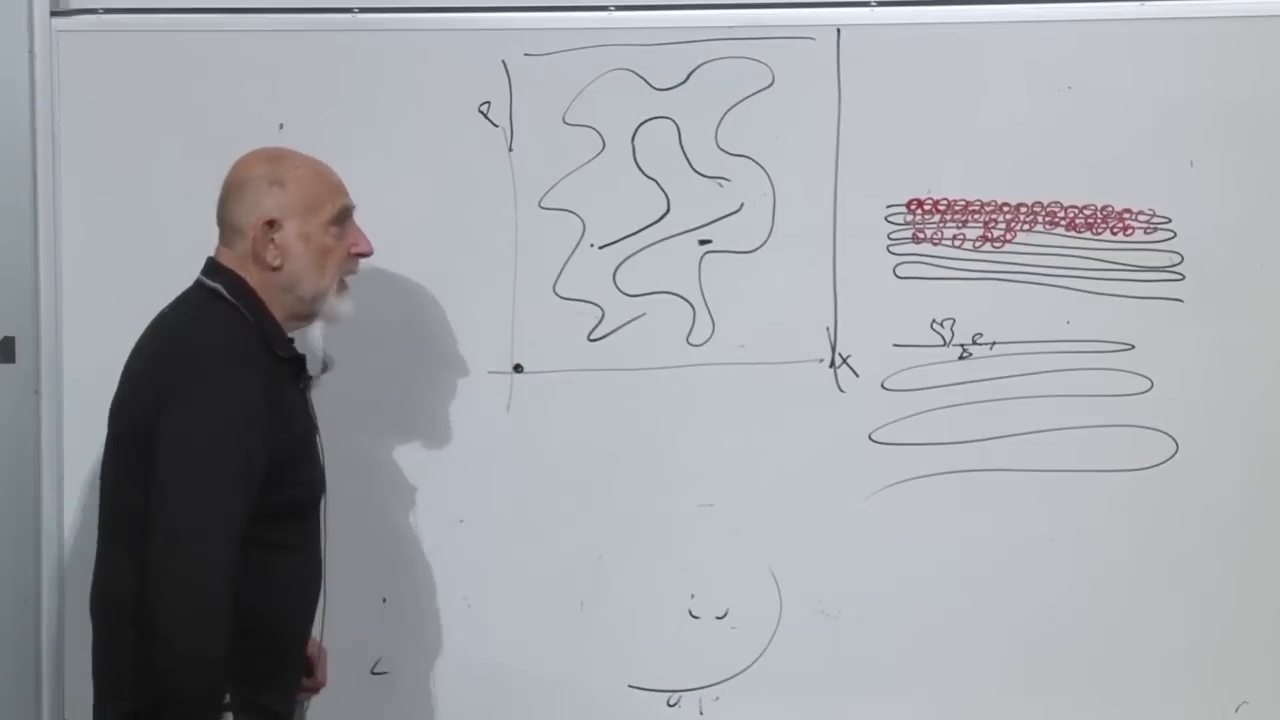
\includegraphics[width=0.90\textwidth]{lecture_07_figure_14.png}
\caption{一个紧致的特殊态在有界的可及区域中演化为复杂的细丝，而粗粒化元胞则散布到远为更大的面积上。}
\lectureframe{01:33:10}
\end{figure}

有两点限定条件很重要。混沌本身并不证明每条轨迹都会访问每个可及邻域；那个更强的采样主张需要遍历性或混合性。也并非每个物理系统都是混沌的。一般的多体气体和理想化台球提供了所设想的场景，在其中混合是一种有用的物理预期。

\section{回归并不消除不可逆性}

假设所有空气分子一开始都位于一个角落，并具有特别制备的速度模式。碰撞很快使它们散布到整个房间，粗粒化描述达到平衡。在有限保测度的相空间中，庞加莱回归定理表明，几乎每个初始点都会任意接近地回到其起点。对于容差\(\epsilon>0\)，在定理的假设下回归时间\(t_R(\epsilon)\)是有限的，尽管对于宏观系统它大得惊人。精确回到一个无限精确的点既非必需，通常也不被预期。

\begin{classroomqa}
\audiencequestion{在台球例子中，击打母球是否会注入能量并破坏封闭演化？}
\lecturerresponse{所选的初始态从击打之后立即开始，那份能量已经包含在内。回归涉及随后孤立的理想化台球动力学；回到初始态附近包括一种构型，其中母球在所选容差内接近球堆。
\lecturetimestamp{01:35:37--01:35:55}}
\end{classroomqa}

\begin{classroomqa}
\audiencequestion{如果气体最终能够回到角落，我们是否丢失了信息，系统是否真的可逆？}
\lecturerresponse{微观动力学始终是可逆的。粗粒化熵可以上升，因为我们不再分辨精细关联，然而一次极其罕见的涨落可以使系统回到其特殊初始宏观态附近。因此，回归与粗粒化不可逆性是相容的。
\lecturetimestamp{01:37:34--01:38:15}}
\end{classroomqa}

这引向玻尔兹曼的基本表述。熵并非在每一个逻辑上可能的瞬间都增加。给定一个大系统的非平衡宏观态，与之相容的微观延续中，压倒性地更多者通向更大的宏观态，而非通向更加特殊的宏观态。熵\emph{很可能}增加。向下的涨落和回归是允许的，但它们的概率和时间尺度使它们在通常的宏观经验中不可见。可逆性问题曾是统计力学历史上重大斗争之一，并沉重地压在玻尔兹曼身上。这一历史关联不应被变成关于他生平的简单因果主张。

\section{混沌意味着什么}

为了给出更具操作性的混沌定义，假设两个初始相点相差\(\delta\Gamma(0)\)，在线性化分离仍有意义的范围内，一个混沌方向通常满足
\begin{equation}
 \lVert\delta\Gamma(t)\rVert
 \sim e^{\lambda t}\lVert\delta\Gamma(0)\rVert,
 \qquad \lambda>0,
 \label{eq:sm7-lyapunov-growth}
\end{equation}
数\(\lambda\)是一个李雅普诺夫指数。要预测时间\(t\)，初始数据所需的精度大致按\(e^{-\lambda t}\)缩放。动力学定律的精度也很重要：模型误差会与初始条件误差一同被放大。天气就是人们熟悉的例子。

\begin{classroomqa}
\audiencequestion{是否存在一条原理，说明\emph{大多数}系统都是混沌的，还是说这仅仅是经验性的？}
\lecturerresponse{混沌与非混沌的哈密顿量都有无穷多个，甚至\emph{大多数}一词也需要在哈密顿量空间上给定一个测度。复杂的相互作用系统往往是混沌的，但并没有一个初等的普适判据，能仅凭检查就把每个哈密顿量分类。
\lecturetimestamp{01:39:27--01:40:49}}
\end{classroomqa}

\begin{classroomqa}
\audiencequestion{在这场讨论中，\emph{混沌}究竟是什么意思？}
\lecturerresponse{邻近的相轨迹分离得足够快，以至于长时间预测要求对初始条件的了解以指数方式改进。谐振子是相反的对照：相邻相点一起旋转并保持接近。精确的两体开普勒问题也是非混沌的，而一般三体问题则存在混沌区域。
\lecturetimestamp{01:40:50--01:43:45}}
\end{classroomqa}

\begin{classroomqa}
\audiencequestion{运动定律以及初始条件都必须知道到高精度吗？}
\lecturerresponse{是的。两种误差来源都会通过动力学传播，而混沌演化会把二者都放大。
\lecturetimestamp{01:43:46--01:43:55}}
\end{classroomqa}

双摆提供了一个生动的例子。普通摆是可积且可预测的。加上第二个摆后，起初几乎一起出发的轨迹最终可能以不同方式转移能量，并朝完全不同的方向运动。

\begin{figure}[t]
\centering
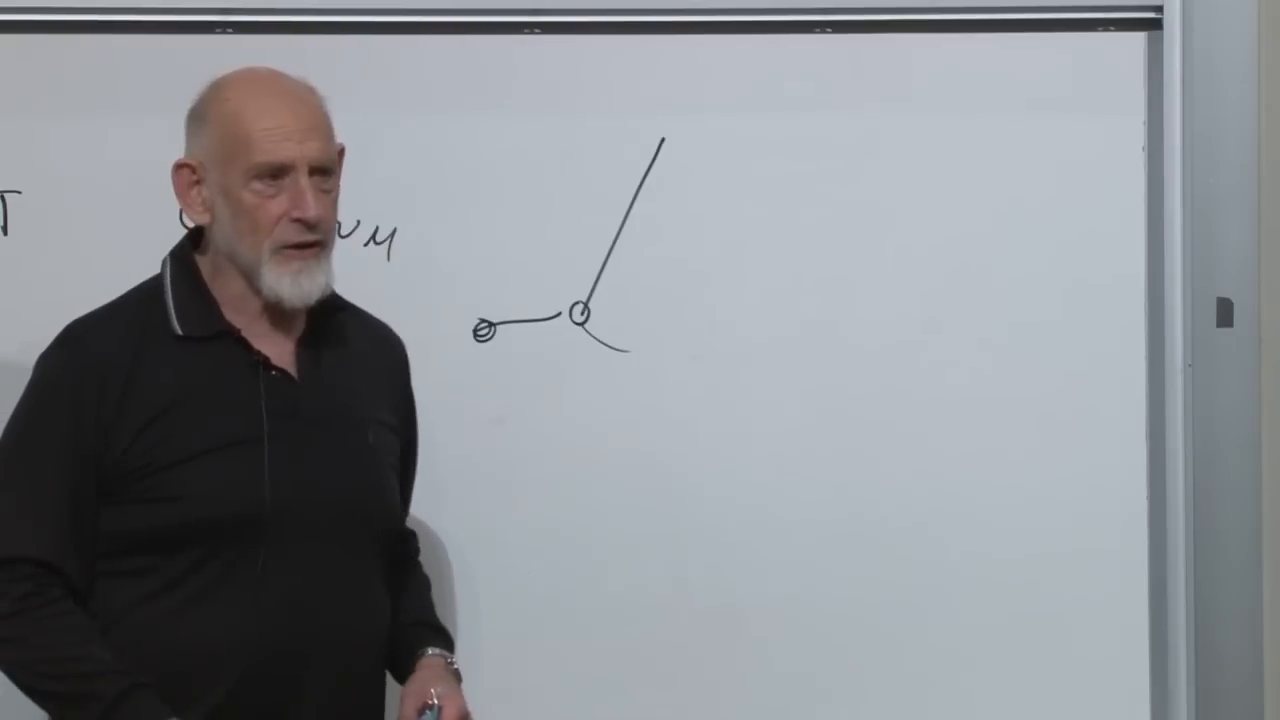
\includegraphics[width=0.90\textwidth]{lecture_07_figure_15.png}
\caption{双摆作为确定性混沌的一个具体例子。}
\lectureframe{01:44:40}
\end{figure}

\begin{classroomqa}
\audiencequestion{为什么一个力学系统可以是混沌的，而另一个却不是？}
\lecturerresponse{这是哈密顿量及其不变结构的性质，而不是摩擦或实验噪声的结果。判定这一点在数学上可能很困难；复杂性有提示作用，但并不是证明。
\lecturetimestamp{01:44:03--01:45:58}}
\end{classroomqa}

\begin{classroomqa}
\audiencequestion{没有摩擦的理想双摆仍然是混沌的吗？}
\lecturerresponse{是的。并不需要耗散。精确的确定性哈密顿运动可以对初始条件具有敏感依赖性。无限精度的初始数据会无限期地确定轨迹，但有限精度给出有限的预测时域。
\lecturetimestamp{01:45:57--01:47:54}}
\end{classroomqa}

\begin{classroomqa}
\audiencequestion{混沌与没有闭式解是同一回事吗？}
\lecturerresponse{不是。混沌系统通常缺乏全局有用的闭式轨迹，但解析可解性与敏感依赖性是两种不同的性质。混沌是通过轨迹分离在动力学上诊断出来的，而不仅仅是因为我们写不出公式。
\lecturetimestamp{01:48:20--01:49:23}}
\end{classroomqa}

\begin{classroomqa}
\audiencequestion{普遍存在的混沌与恰好平衡在不稳定的山顶上有什么不同？}
\lecturerresponse{山顶是一个例外的不稳定状态：离开它以后，邻近轨迹未必会迅速分离。在混沌区域中，不稳定性沿轨道是典型的，邻近相点会反复分离。正的李雅普诺夫指数刻画了这种持续增长。
\lecturetimestamp{01:49:27--01:50:11}}
\end{classroomqa}

\section{从微观运动到统计定律}

声速估计表明，微观热运动如何确定一个宏观传播尺度，而其中的问题则揭示出必须指定哪个热力学导数。随后，振子展示了经典能量均分所能达到的范围及其失效。量子能级间距冻结了刚性模式，解释了热容为何随温度变化，并阻止无穷多个高频模式携带无穷大的热能。

从精确的微观物理到有效宏观描述的同一递进过程，化解了第二定律核心处的表面矛盾。哈密顿流保持精确的相空间体积并且保持可逆。混沌拉伸产生的关联比宏观描述所保留的更精细，因此粗粒化后的占据区域会增长。回归性保证罕见的返回并非被禁止；概率解释了为什么它们不构成日常经验。第二定律并不是一种新的不可逆微观力。对于具有极多自由度的系统中特殊的宏观初始条件，它是演化过程压倒性地可靠的统计方向。